%=====================================================================
%  SHARED PREAMBLE — Quantitative Reasoning LAB 413 Beamer theme
%  Paste this block VERBATIM at the top of every LabN_beamer.tex
%  (keep each deck self-contained; do NOT \input this file).
%  Compile: pdflatex LabN_beamer.tex   (run twice for footline counters)
%=====================================================================
\documentclass[aspectratio=169,11pt]{beamer}

\usepackage[utf8]{inputenc}
\usepackage[T1]{fontenc}
\usepackage{lmodern}
\usepackage{amsmath,amssymb}
\usepackage{graphicx}
\usepackage{booktabs}
\usepackage{tcolorbox}
\tcbuselibrary{skins}

\usetheme{default}
\usecolortheme{default}
\useinnertheme{circles}

\definecolor{qrnavy}{RGB}{20,44,90}
\definecolor{qrblue}{RGB}{38,80,150}
\definecolor{qrgray}{RGB}{90,95,105}
\definecolor{qrlight}{RGB}{234,239,247}
\definecolor{qrred}{RGB}{190,60,60}

\setbeamercolor{structure}{fg=qrnavy}
\setbeamercolor{frametitle}{fg=white,bg=qrnavy}
\setbeamercolor{title}{fg=qrnavy}
\setbeamercolor{block title}{fg=white,bg=qrblue}
\setbeamercolor{block body}{bg=qrlight}
\setbeamercolor{itemize item}{fg=qrblue}
\setbeamercolor{itemize subitem}{fg=qrblue}
\setbeamerfont{frametitle}{series=\bfseries}
\setbeamertemplate{navigation symbols}{}

\setbeamertemplate{frametitle}{%
  \nointerlineskip
  \begin{beamercolorbox}[wd=\paperwidth,ht=3.2ex,dp=1.2ex,leftskip=0.3cm]{frametitle}%
    \strut\insertframetitle\strut
  \end{beamercolorbox}%
}

% Footline: course | lab N | slide number  (edit "Lab N" per deck)
\newcommand{\labnum}{Lab 8}   % <-- SET THIS to the lab number, e.g. \renewcommand{\labnum}{Lab 3}
\setbeamertemplate{footline}{%
  \leavevmode%
  \hbox{%
    \begin{beamercolorbox}[wd=.5\paperwidth,ht=2.4ex,dp=1ex,leftskip=.3cm]{author in head/foot}%
      \usebeamerfont{author in head/foot}\color{qrgray}\small Quantitative Reasoning -- LAB 413%
    \end{beamercolorbox}%
    \begin{beamercolorbox}[wd=.5\paperwidth,ht=2.4ex,dp=1ex,rightskip=.3cm]{title in head/foot}%
      \usebeamerfont{title in head/foot}\color{qrgray}\small\hfill \labnum \quad\insertframenumber\,/\,\inserttotalframenumber%
    \end{beamercolorbox}}%
}

% Number badge (01, 02, ...) used on concept slides:  \numbadge{01}
\newtcbox{\numbadge}{on line,boxsep=2pt,left=4pt,right=4pt,top=2pt,bottom=2pt,
  colback=qrnavy,colframe=qrnavy,fontupper=\bfseries\color{white},arc=2pt}

% Key-concepts callout:  \begin{keybox} ... \end{keybox}   or  \begin{keybox}[Scenario] ...
\newtcolorbox{keybox}[1][Key Concepts]{colback=qrlight,colframe=qrnavy,
  fonttitle=\bfseries,title={#1},coltitle=white,arc=2pt,left=4pt,right=4pt,
  top=3pt,bottom=3pt,boxrule=0.6pt}

%---------------------------------------------------------------------
%  Title data
%---------------------------------------------------------------------
\title{\bfseries t-Distributions \& Inferences for Means}
\subtitle{Week 9 Recap \textbullet\ Lab 8}
\author{Instructor: Subin Na}
\institute{Quantitative Reasoning -- LAB 413}
\date{October 29, 2025}

\begin{document}

%---------------------------------------------------------------------
%  Title slide
%---------------------------------------------------------------------
{\setbeamertemplate{footline}{}
\begin{frame}
  \vfill
  {\color{qrgray}\small Quantitative Reasoning -- LAB 413}\\[0.6em]
  {\usebeamerfont{title}\color{qrnavy}\huge\bfseries t-Distributions\\[0.15em]\& Inferences for Means\par}
  \vspace{0.4em}
  {\color{qrblue}\large Week 9 Recap \ \textbullet\ \ Lab 8}\par
  \vspace{1.6em}
  {\color{qrgray} Instructor: \textbf{Subin Na} \hfill October 29, 2025}
  \vfill
\end{frame}
}

%---------------------------------------------------------------------
%  Today's Plan
%---------------------------------------------------------------------
\begin{frame}{Today's Plan}
  \begin{columns}[T]
    \begin{column}{0.5\textwidth}
      \textbf{\color{qrnavy}1. Quick Recap}
      \begin{itemize}
        \item Categorical Variables in Regression
        \item t-Distributions Overview
        \item t Confidence Interval
        \item Matched Pairs
        \item Comparing Two Means
      \end{itemize}
    \end{column}
    \begin{column}{0.5\textwidth}
      \phantom{\textbf{x}}
      \vspace{2.4em}

      \textbf{\color{qrnavy}2. RStudio Practice}
    \end{column}
  \end{columns}
\end{frame}

%---------------------------------------------------------------------
%  01 Categorical Variables in Regression
%---------------------------------------------------------------------
\begin{frame}{\numbadge{01}\ \ Categorical Variables in Regression}
  \begin{itemize}
    \item Quantitative models need numeric predictors $\rightarrow$ \textbf{dummy variables}.
    \item Create binary indicators for each category (omit one $\rightarrow$ avoid the ``dummy variable trap'').
  \end{itemize}
  \vspace{0.4em}
  \begin{keybox}[Example]
    \begin{equation*}
      \text{turnout}_i = \alpha + \beta_1\,\text{Republican}_i + \beta_2\,\text{Independent}_i + \varepsilon_i
    \end{equation*}
  \end{keybox}
  \vspace{0.3em}
  \textbf{\color{qrnavy}Interpretation}
  \begin{itemize}
    \item $\hat{\alpha}$ = mean turnout for the reference group (e.g., Democrats).
    \item $\hat{\beta}$ = difference in means vs.\ the reference group.
  \end{itemize}
\end{frame}

%---------------------------------------------------------------------
%  02 t-Distributions Overview (1)
%---------------------------------------------------------------------
\begin{frame}{\numbadge{02}\ \ t-Distributions Overview (1)}
  \begin{columns}[T]
    \begin{column}{0.46\textwidth}
      \textbf{\color{qrnavy}Use when:}
      \begin{itemize}
        \item Sample size $n < 30$
        \item Population $\sigma$ unknown
      \end{itemize}
      \vspace{0.3em}
      \begin{itemize}
        \item Replace $z$ with $t$, $\sigma$ with $s_x$.
        \item Degrees of freedom (df) $= n - 1$.
        \item $t$ has fatter tails than Normal $\rightarrow$ more uncertainty with small $n$.
        \item As $n \rightarrow \infty$, $t \rightarrow$ Normal.
      \end{itemize}
    \end{column}
    \begin{column}{0.54\textwidth}
      \centering
      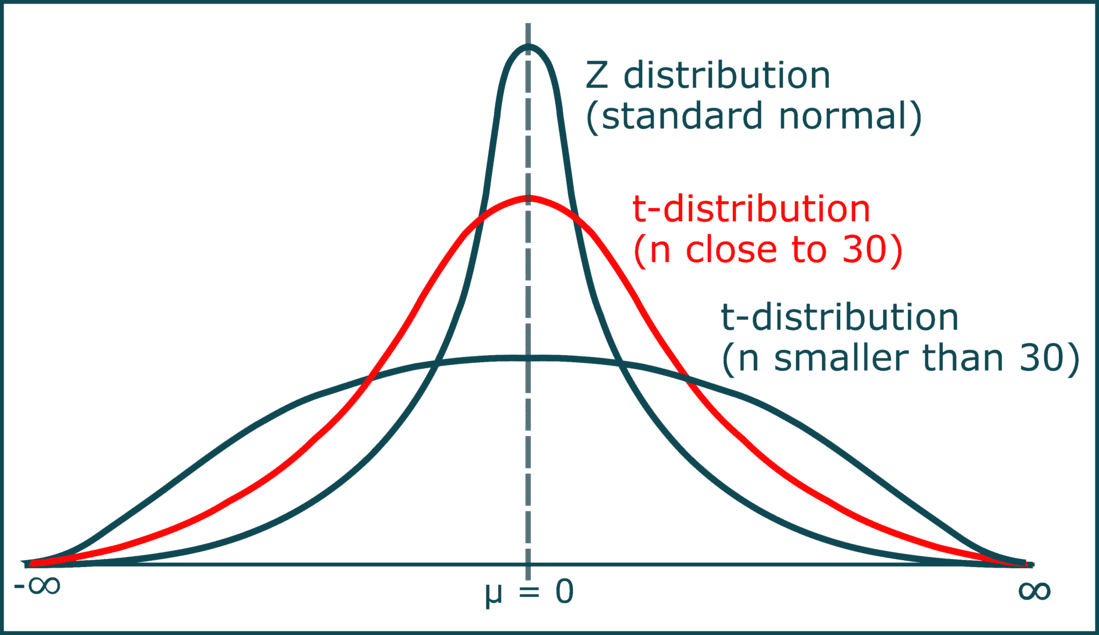
\includegraphics[width=\textwidth]{figures/s04_3_6.8x3.9.png}
    \end{column}
  \end{columns}
\end{frame}

%---------------------------------------------------------------------
%  02 t-Distributions Overview (2)
%---------------------------------------------------------------------
\begin{frame}{\numbadge{02}\ \ t-Distributions Overview (2)}
  \textbf{\color{qrnavy}Before applying $t$-procedures, check:}
  \begin{enumerate}
    \item \textbf{Random sampling:} data should come from a random sample.
    \item \textbf{Normality assumption:} is it reasonable to assume the population is roughly Normal?
  \end{enumerate}
  \vspace{0.4em}
  \begin{keybox}[Sample distribution]
    \begin{itemize}
      \item If $n < 30$, check that data are roughly symmetric with no outliers.
      \item If $n < 15$, don't use $t$-procedures if data are skewed or contain outliers.
      \item If $n \geq 40$, $t$-procedures are robust even with some skew.
    \end{itemize}
  \end{keybox}
\end{frame}

%---------------------------------------------------------------------
%  03 t Confidence Interval
%---------------------------------------------------------------------
\begin{frame}{\numbadge{03}\ \ t Confidence Interval}
  \textbf{\color{qrnavy}Steps to calculate}
  \begin{enumerate}
    \item Verify conditions (random sample; approx.\ normal data, no strong skew/outliers).
    \item Identify given values.
    \item Find the critical $t$-value $t^*$ from the $t$-table (based on confidence level \& df).
    \item Compute the confidence interval using the formula.
    \item Interpret the interval in context (e.g., ``We are 95\% confident that the true mean lies between \_\_\_ and \_\_\_'').
  \end{enumerate}
  \vspace{0.2em}
  \begin{equation*}
    \bar{x} \;\pm\; t^* \,\frac{s_x}{\sqrt{n}}
  \end{equation*}
\end{frame}

%---------------------------------------------------------------------
%  Example: study hours
%---------------------------------------------------------------------
\begin{frame}{Example: Study Hours}
  \begin{keybox}[Scenario]
    A researcher wants to estimate the average number of hours Penn students study
    per week. She collects a simple random sample of \textbf{25 students} and finds:
    \begin{itemize}
      \item Sample mean $= 14.2$ hours
      \item Sample standard deviation $= 4.5$ hours
    \end{itemize}
    Assume the data are roughly symmetric with no clear outliers.
  \end{keybox}
  \vspace{0.5em}
  \begin{center}
    Construct a 95\% confidence interval for the true mean study hours per week,
    and interpret the interval in context.
  \end{center}
\end{frame}

%---------------------------------------------------------------------
%  t Table (reference)
%---------------------------------------------------------------------
\begin{frame}{Reference: t Table}
  \begin{center}
    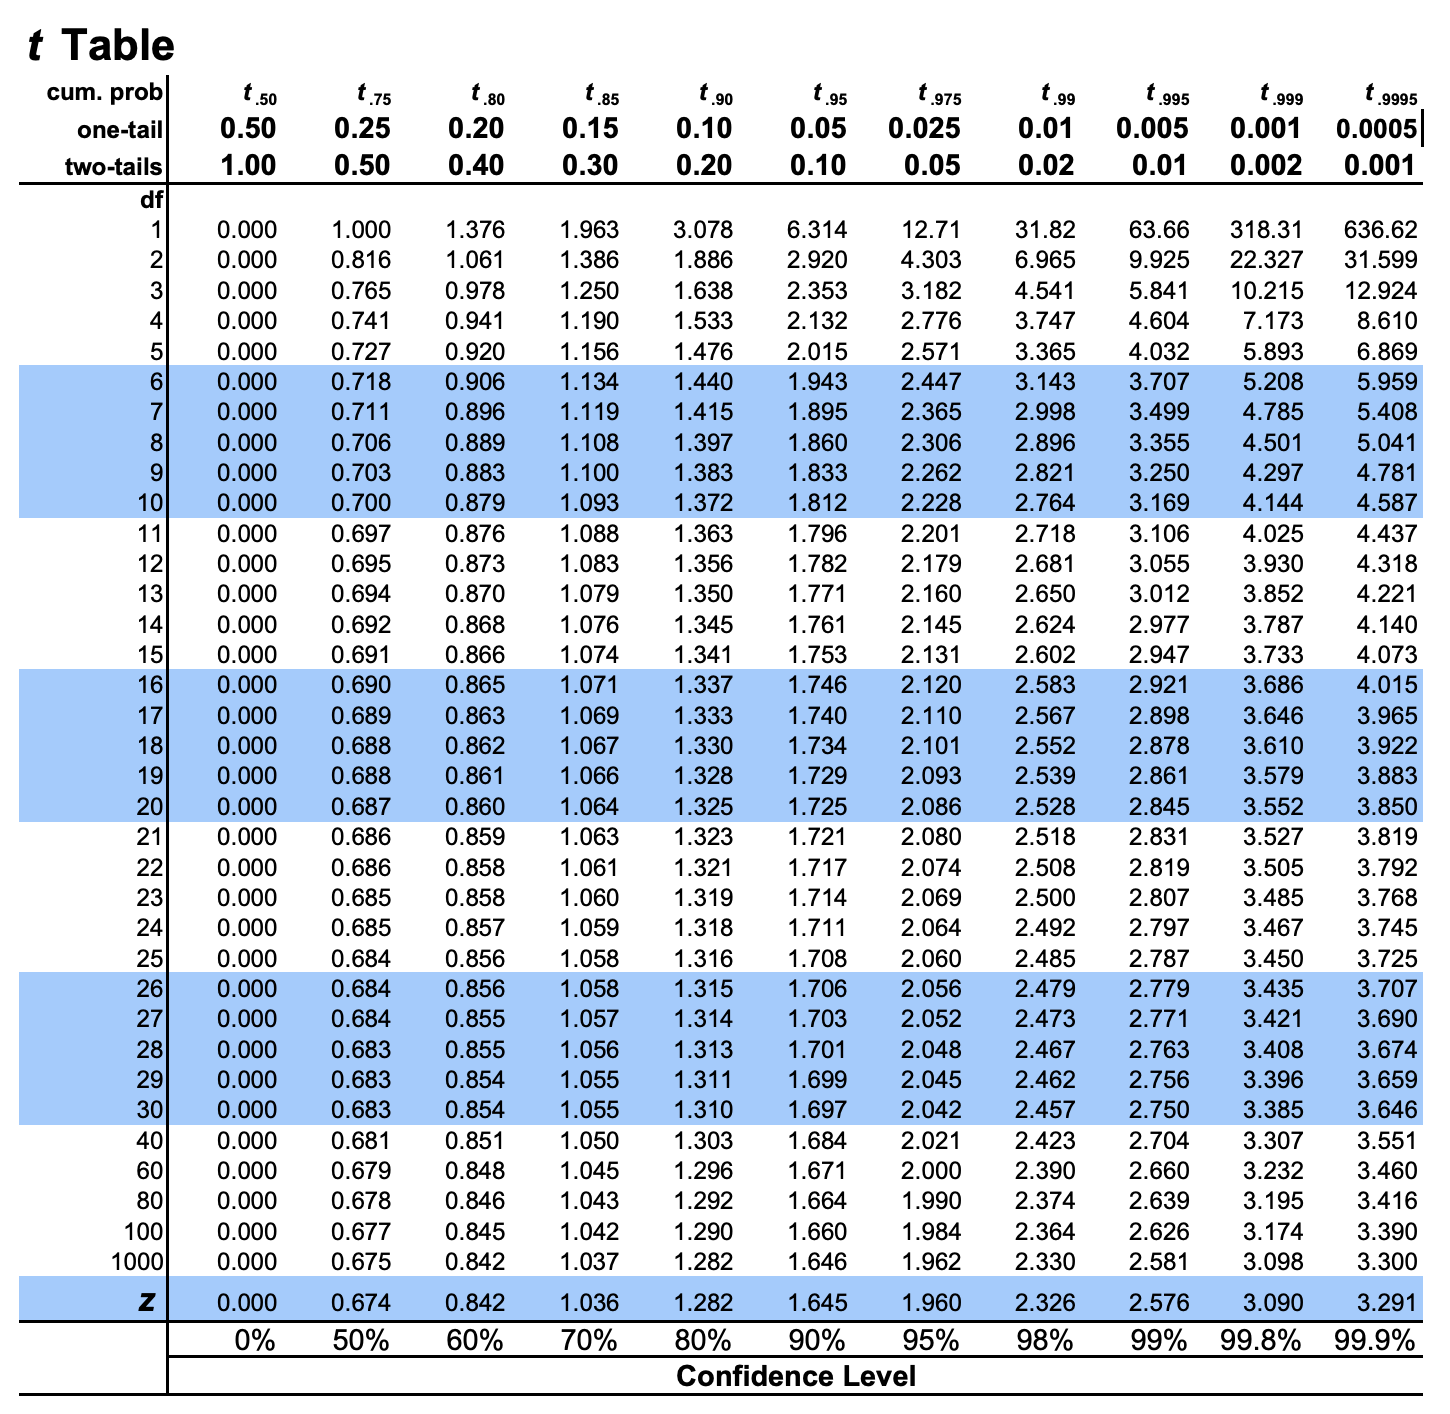
\includegraphics[height=0.78\textheight]{figures/s08_1_11.3x11.0.png}\\[0.2em]
    {\scriptsize\color{qrgray}Source: sjsu.edu/faculty/gerstman/StatPrimer/t-table.pdf}
  \end{center}
\end{frame}

%---------------------------------------------------------------------
%  Solution: study hours
%---------------------------------------------------------------------
\begin{frame}{Solution: Study Hours}
  \small
  \begin{columns}[T]
    \begin{column}{0.38\textwidth}
      \textbf{\color{qrnavy}Given}
      \begin{align*}
        \bar{x} &= 14.2\\
        s_x &= 4.5\\
        n &= 25\\
        df &= 24
      \end{align*}
      95\% confidence $\rightarrow t^* = 2.064$
    \end{column}
    \begin{column}{0.62\textwidth}
      \textbf{\color{qrnavy}Compute}
      \begin{align*}
        \text{CI} &= 14.2 \pm 2.064 \times \frac{4.5}{\sqrt{25}}\\
                  &= 14.2 \pm 2.064 \times 0.9\\
                  &= 14.2 \pm 1.86\\
        \Rightarrow \text{CI} &= [\,12.34,\ 16.06\,]
      \end{align*}
      \begin{tcolorbox}[colback=qrlight,colframe=qrnavy,arc=2pt,boxrule=0.6pt]
        \footnotesize We are 95\% confident that the true mean study hours per week
        among Penn students lies between \textbf{12.34} and \textbf{16.06} hours.
      \end{tcolorbox}
    \end{column}
  \end{columns}
\end{frame}

%---------------------------------------------------------------------
%  04 Matched Pairs (1)
%---------------------------------------------------------------------
\begin{frame}{\numbadge{04}\ \ Matched Pairs (1)}
  \textbf{\color{qrnavy}When do we use matched pairs?}
  \begin{itemize}
    \item Same subjects measured twice (before--after), or
    \item Two matched individuals (e.g., twins, pairs in an experiment).
    \item We analyze the \textbf{differences as one sample}.
  \end{itemize}
  \vspace{0.4em}
  \begin{keybox}
    \begin{itemize}
      \item \textbf{Goal:} determine whether the mean of the differences is significantly different from $0$.
      \item If CI includes $0 \rightarrow$ no significant difference.
      \item If CI excludes $0 \rightarrow$ significant difference in means.
    \end{itemize}
  \end{keybox}
\end{frame}

%---------------------------------------------------------------------
%  04 Matched Pairs (2)
%---------------------------------------------------------------------
\begin{frame}{\numbadge{04}\ \ Matched Pairs (2)}
  \textbf{\color{qrnavy}Steps for a matched-pair $t$-test / $t$-interval}
  \begin{enumerate}
    \item Calculate the difference for each pair: $\quad d_i = X_{1i} - X_{2i}$
    \item Compute the mean and SD of the differences.
    \item Use one-sample $t$-procedures on $d_i$.
    \item Build the CI using
      \begin{equation*}
        \bar{d} \;\pm\; t^* \,\frac{s_d}{\sqrt{n}}
      \end{equation*}
    \item Interpret: if CI includes $0 \rightarrow$ no significant difference.
  \end{enumerate}
\end{frame}

%---------------------------------------------------------------------
%  Example: online vs in-class quiz
%---------------------------------------------------------------------
\begin{frame}{Example: Online vs.\ In-Class Quiz}
  \begin{columns}[T]
    \begin{column}{0.52\textwidth}
      A professor wants to test whether SP2 students score differently on two types
      of quizzes: \textbf{online} vs.\ \textbf{in-class}. Five students took both
      versions, with scores (out of 10):
      \vspace{0.4em}

      $d_i = \text{Online} - \text{In-Class}$
      \vspace{0.6em}

      \textbf{\color{qrnavy}Tasks}
      \begin{itemize}
        \item Construct a 95\% CI for the true mean difference.
        \item Interpret: do the two quiz formats lead to significantly different scores?
      \end{itemize}
    \end{column}
    \begin{column}{0.44\textwidth}
      \centering
      \renewcommand{\arraystretch}{1.2}
      \begin{tabular}{@{}ccc@{}}
        \toprule
        \textbf{Student} & \textbf{Online} & \textbf{In-Class}\\
        \midrule
        1 & 8  & 7\\
        2 & 6  & 6\\
        3 & 9  & 8\\
        4 & 7  & 7\\
        5 & 10 & 9\\
        \bottomrule
      \end{tabular}
    \end{column}
  \end{columns}
\end{frame}

%---------------------------------------------------------------------
%  t Table (reference, again)
%---------------------------------------------------------------------
\begin{frame}{Reference: t Table}
  \begin{center}
    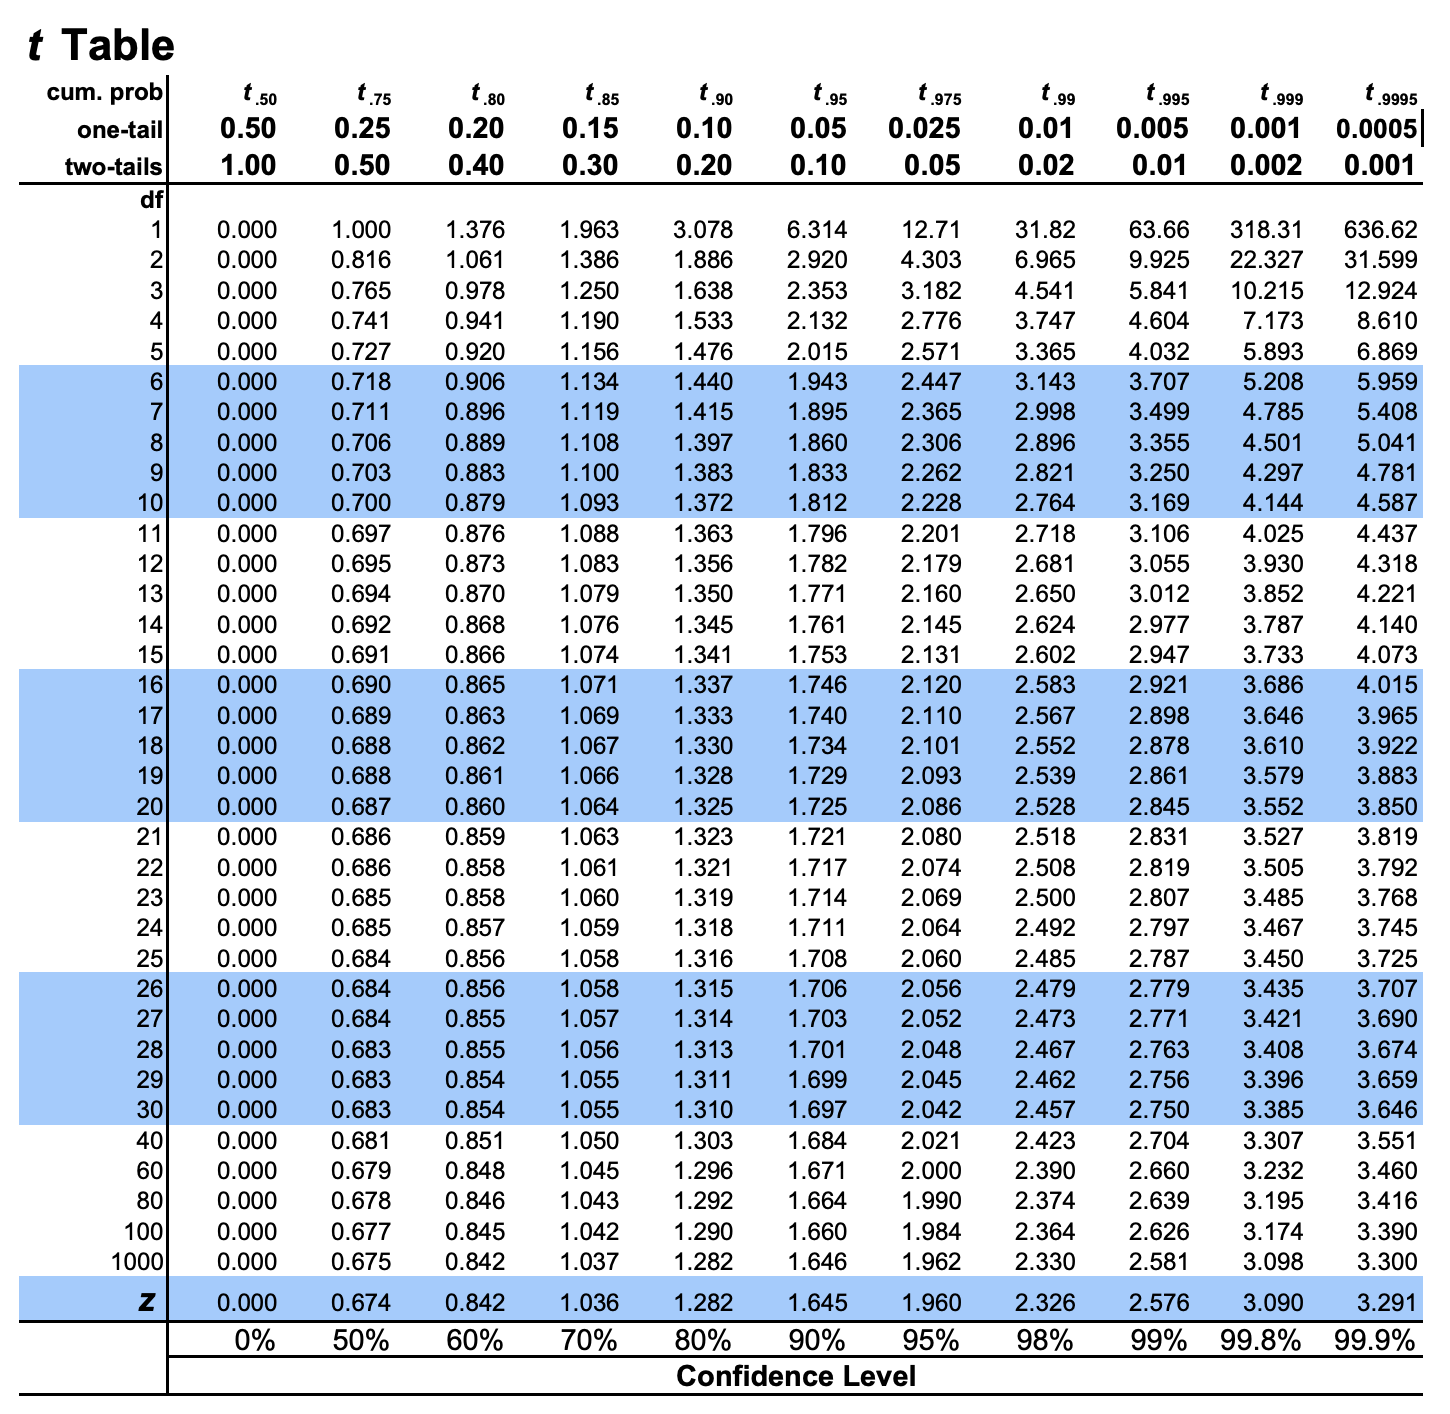
\includegraphics[height=0.78\textheight]{figures/s13_1_11.3x11.0.png}\\[0.2em]
    {\scriptsize\color{qrgray}Source: sjsu.edu/faculty/gerstman/StatPrimer/t-table.pdf}
  \end{center}
\end{frame}

%---------------------------------------------------------------------
%  Solution (1): compute differences & summary stats
%---------------------------------------------------------------------
\begin{frame}{Solution: Online vs.\ In-Class (1)}
  \small
  \textbf{\color{qrnavy}Step 1. Compute differences}
  \begin{equation*}
    d = [\,1,\ 0,\ 1,\ 0,\ 1\,]
  \end{equation*}
  \textbf{\color{qrnavy}Step 2. Summary statistics}
  \begin{align*}
    \bar{d} &= \frac{1+0+1+0+1}{5} = 0.6\\[0.4em]
    d_i - \bar{d} &= [\,0.4,\ -0.6,\ 0.4,\ -0.6,\ 0.4\,]\\
    (d_i - \bar{d})^2 &= [\,0.16,\ 0.36,\ 0.16,\ 0.36,\ 0.16\,]
        \quad\Rightarrow\quad \textstyle\sum (d_i-\bar{d})^2 = 1.20\\[0.4em]
    s_d &= \sqrt{\frac{\sum_{i=1}^{n}(d_i-\bar{d})^2}{n-1}}
         = \sqrt{\frac{1.20}{5-1}} = \sqrt{0.30} \approx 0.548
  \end{align*}
\end{frame}

%---------------------------------------------------------------------
%  Solution (2): construct CI & interpret
%---------------------------------------------------------------------
\begin{frame}{Solution: Online vs.\ In-Class (2)}
  \small
  \textbf{\color{qrnavy}Step 3. Construct CI}\quad ($n = 5,\ df = 4,\ 95\%$ confidence $\rightarrow t^* = 2.776$)
  \begin{align*}
    \text{CI} &= 0.6 \pm 2.776 \times \frac{0.548}{\sqrt{5}}\\
              &= 0.6 \pm 0.68\\
    \Rightarrow \text{CI} &= [\,-0.08,\ 1.28\,]
  \end{align*}
  \vspace{0.2em}
  \textbf{\color{qrnavy}Step 4. Interpretation}
  \begin{tcolorbox}[colback=qrlight,colframe=qrred,arc=2pt,boxrule=0.6pt]
    Since the 95\% CI \textbf{includes 0}, there is no statistically significant
    difference between online and in-class quiz scores.
  \end{tcolorbox}
\end{frame}

%---------------------------------------------------------------------
%  05 Comparing Two Means
%---------------------------------------------------------------------
\begin{frame}{\numbadge{05}\ \ Comparing Two Means}
  \begin{itemize}
    \item Used when there are two \textbf{independent} samples (e.g., treatment vs.\ control).
    \item Each group's observations are independent.
    \item \textbf{Interpretation:} the difference in sample means estimates the
          difference between population means (causal if randomized).
    \item Common in experimental or policy-evaluation settings (e.g., program
          participants vs.\ nonparticipants).
  \end{itemize}
  \vspace{0.6em}
  \begin{keybox}[Two-sample $t$ confidence interval]
    \begin{equation*}
      (\bar{x}_T - \bar{x}_C) \;\pm\; t^* \sqrt{\frac{s_T^2}{n_T} + \frac{s_C^2}{n_C}}
    \end{equation*}
  \end{keybox}
\end{frame}

%---------------------------------------------------------------------
%  Transition to RStudio
%---------------------------------------------------------------------
{\setbeamertemplate{footline}{}
\begin{frame}
  \vfill
  \centering
  {\color{qrnavy}\Huge\bfseries RStudio Practice}\\[0.8em]
  {\color{qrblue}\large $t$-tests \& Categorical Variables}\\[0.4em]
  {\color{qrgray} See \texttt{Lab8.Rmd} / \texttt{Lab8\_1029.R}}
  \vfill
\end{frame}
}

\end{document}
